% arara: pdflatex
% arara: pdflatex
\documentclass[12pt]{article}
\usepackage{amsmath, amssymb}
\usepackage{fullpage}
\usepackage{float}
\usepackage{mathptmx}
\usepackage{fancyvrb}
\usepackage{graphicx}
\usepackage{caption}
\usepackage{subcaption}
\usepackage{multirow}
\usepackage{listings}
\usepackage{helvet}
\usepackage{microtype}
\usepackage{booktabs} %enhancements to tables
\usepackage{tablefootnote} %footnotes in tables
\usepackage{multirow} %span rows in tables
\usepackage{tabu}
\usepackage{xcolor}
\usepackage{cleveref}
\usepackage{units}
\usepackage{titling}

\renewcommand*\familydefault{\sfdefault}

\pretitle{\begin{flushleft}\LARGE}
\posttitle{\par\end{flushleft}}
\preauthor{\begin{flushleft}\large}
\postauthor{\par\end{flushleft}}
\predate{\begin{flushleft}\large}
\postdate{\par\end{flushleft}}

\newcommand{\e}{\ensuremath{ \mbox{\small{E}} }}

\title{\sc NE770 HW 1}
\author{Jason M. Hite}
\date{}

%adjust booktab heavy rule width
\setlength\heavyrulewidth{2pt}

% Fix mathcal font
\DeclareMathAlphabet{\mathcal}{OMS}{cmsy}{m}{n}

\begin{document}

\maketitle

The code accompanying this report can be found at . The source for this report and for generation of the
plots can be viewed here.

\section*{Problem 1}

This problem is to evaluate the following integral via simple Monte Carlo.
\begin{equation}
    \int_0^\pi \theta\sin(\theta)d\theta
    \label{eq:montint}
\end{equation}
Using 2000 samples, the Monte Carlo estimate for the integral in~\cref{eq:montint} is 3.1261762, with an
error variance of $\hat\sigma^2=\sigma^2/N=.0019117841$. The actual value for~\cref{eq:montint} evaluates to $\pi\approx
3.1415927$, which is an error of $-.01541650$ and is less than $\hat\sigma = .0437239534$. \Cref{fig:1} shows the mean,
variance and error variance for the Monte Carlo estimate of~\cref{eq:montint} as a function of the number of samples $N$.
It can be seen in~\cref{fig:1:mu,fig:1:var} that the estimates for the integral and the variances stabilize around $N>500$,
while~\cref{fig:1:err} indicates that the solution is accurate to two significant figures starting around $N>200$.

\begin{figure}[H]
    \centering
    \begin{subfigure}[b]{.49\textwidth}
        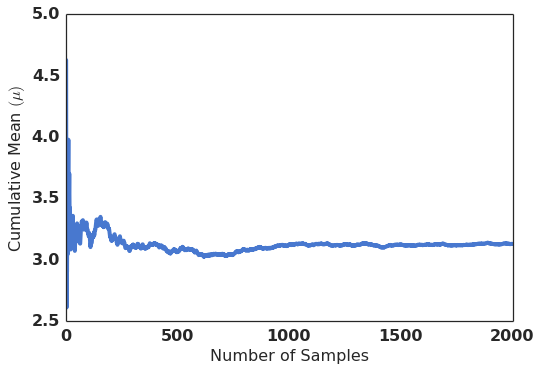
\includegraphics[width=\textwidth]{fig/1mu.png}
        \caption{Cumulative mean}
        \label{fig:1:mu}
    \end{subfigure}
    \begin{subfigure}[b]{.49\textwidth}
        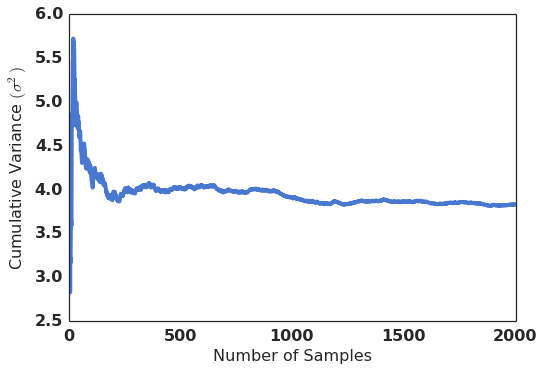
\includegraphics[width=\textwidth]{fig/1var.png}
        \caption{Cumulative variance}
        \label{fig:1:var}
    \end{subfigure}
    \begin{subfigure}[b]{.49\textwidth}
        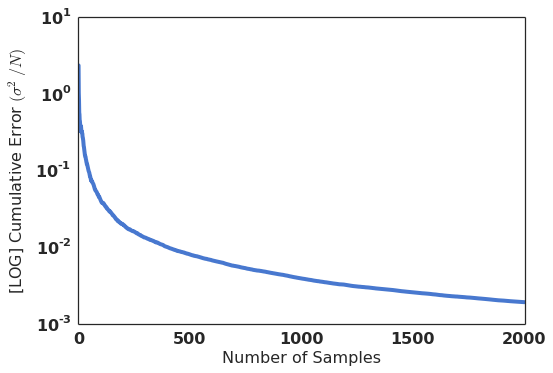
\includegraphics[width=\textwidth]{fig/1err.png}
        \caption{Cumulative error (log scale)}
        \label{fig:1:err}
    \end{subfigure}
    \caption{Plots of $\mu$, $\sigma^2$ and $\sigma^2 / N$ with increasing number of samples}
    \label{fig:1}
\end{figure}

\section*{Problem 2}

Here, we attempt to sample the following functions:
\begin{equation}
    \chi(E) = .453\exp(-E/.965)\sinh(2.29)^\frac{1}{2}
    \label{eq:chi}
\end{equation}
\begin{equation}
    \nu(E) = 
    \begin{cases}
        2.42 + .066E, & E\leq 1 \\
        2.349 + .15E, & E > 1
    \end{cases}
    \label{eq:nu}
\end{equation}
\Cref{eq:chi} describes the energy spectrum of fission neutrons and is a probability density, while~\cref{eq:nu}
gives the average number of neutrons emitted per fission initiated at energy $E$ and is proportional to a probability
density. Both are defined for the half-open interval $E\in [0,\infty)$; we seek to determine the mean fission
neutron energy and the mean number of neutrons released per fission. By definition, the mean $\mu$ for a given (potentially
un-normalized) probability distribution $p(x)$ with support $\mathcal{D}$ can be computed via the relation:
\begin{equation}
    \mu = \frac{\int_\mathcal{D} x \cdot p(x) dx}{\int_\mathcal{D} p(x) dx}
    \label{eq:meanexpr}
\end{equation}
We first apply~\cref{eq:meanexpr} to~\cref{eq:chi,eq:nu} and evaluate numerically using an adaptive Gauss-Kronrod
quadrature implemented in QUADPACK. This produces the values in~\cref{tab:quad}, which serve as reference values to compare
the sampling methods against.
\begin{table}[H]
    \centering
    \begin{tabular}{lcc}
        \toprule
          & $\mu$ & Quadrature error \\
        \midrule
        $\chi(E)$ & $1.9819186$ & $2.2991644\e-8$ \\
        $\nu(E)$ & $5.3985461$ & $2.4323015\e-9$ \\
        \bottomrule
    \end{tabular}
    \caption{Means for $\chi$ and $\nu$ evaluated by quadrature}
    \label{tab:quad}
\end{table}

\end{document}
